\chapter{Acides et bases — pH, couples acide/base, \texorpdfstring{$\mathbf{pK_a}$}{pKa}}

\textit{La notion d'acide et de base est fondamentale en chimie. De la simple réaction entre le vinaigre et la soude jusqu'aux processus biologiques complexes (digestion, respiration), les réactions acido-basiques sont omniprésentes. Ce chapitre pose les bases de la théorie de Brønsted, introduit les outils quantitatifs que sont le pH, le $K_a$ et le $pK_a$, et vous apprend à calculer le pH de solutions d'acides et de bases, qu'ils soient forts ou faibles.}

% ====================================================================
\section{Théorie de Brønsted — Définitions fondamentales}
% ====================================================================

\begin{definition}[Acide et base selon Brønsted]
Un \textbf{acide} est une espèce chimique capable de \textbf{céder} un proton $\ce{H+}$.
Une \textbf{base} est une espèce chimique capable de \textbf{capter} un proton $\ce{H+}$.
\end{definition}

\begin{exemple}
\begin{itemize}
    \item L'acide chlorhydrique $\ce{HCl}$ est un acide : $\ce{HCl -> H+ + Cl-}$.
    \item L'ammoniac $\ce{NH3}$ est une base : $\ce{NH3 + H+ -> NH4+}$.
    \item L'ion hydrogénocarbonate $\ce{HCO3-}$ peut se comporter comme un acide ou une base (amphotère).
\end{itemize}
\end{exemple}

\begin{definition}[Couple acide/base]
Un \textbf{couple acide/base} est constitué de deux espèces chimiques qui ne diffèrent que par un proton $\ce{H+}$. On le note $\text{acide}/\text{base}$.
\[
\ce{Acide <=> Base + H+}
\]
\end{definition}

\begin{exemple}
Quelques couples acide/base importants :
\begin{itemize}
    \item $\ce{HCl / Cl-}$ (acide chlorhydrique / ion chlorure)
    \item $\ce{CH3COOH / CH3COO-}$ (acide éthanoïque / ion éthanoate)
    \item $\ce{NH4+ / NH3}$ (ion ammonium / ammoniac)
    \item $\ce{H2O / HO-}$ (eau / ion hydroxyde)
    \item $\ce{H3O+ / H2O}$ (ion oxonium / eau)
\end{itemize}
\end{exemple}

\begin{definition}[Réaction acido-basique]
Une \textbf{réaction acido-basique} est une réaction chimique au cours de laquelle il y a \textbf{transfert d'un proton} $\ce{H+}$ d'un acide vers une base.
\[
\ce{Acide1 + Base2 <=> Base1 + Acide2}
\]
\end{definition}

\begin{experience}[Réaction entre l'acide chlorhydrique et l'ammoniac]
Dans un bécher, on verse une solution d'acide chlorhydrique $\ce{HCl_{(aq)}}$ et on ajoute une solution d'ammoniac $\ce{NH3_{(aq)}}$. On observe un dégagement de chaleur (réaction exothermique). L'équation de la réaction est :
\[
\ce{HCl_{(aq)} + NH3_{(aq)} -> NH4+_{(aq)} + Cl-_{(aq)}}
\]
L'acide $\ce{HCl}$ a cédé un proton à la base $\ce{NH3}$.
\end{experience}

\begin{remarque}
Un proton $\ce{H+}$ n'existe pas libre en solution aqueuse ; il est immédiatement hydraté pour former l'ion oxonium $\ce{H3O+}$. L'écriture $\ce{H+}$ est une simplification commode.
\end{remarque}

% ====================================================================
\section{Autoprotolyse de l'eau — Produit ionique de l'eau}
% ====================================================================

\begin{definition}[Autoprotolyse de l'eau]
L'eau pure est le siège d'une réaction d'équilibre appelée \textbf{autoprotolyse} : une molécule d'eau cède un proton à une autre molécule d'eau.
\[
\ce{2 H2O <=> H3O+ + HO-}
\]
\end{definition}

\begin{loi}[Produit ionique de l'eau $K_e$]
À une température donnée, le produit des concentrations des ions oxonium et hydroxyde dans l'eau pure (ou dans toute solution aqueuse diluée) est constant. On l'appelle le \textbf{produit ionique de l'eau}, noté $K_e$.
\[
K_e = [\ce{H3O+}] \times [\ce{HO-}]
\]
À $\SI{25}{\celsius}$, $K_e = \num{1.0e-14}$.
\end{loi}

\begin{propriete}[Conséquences]
\begin{itemize}
    \item Dans l'eau pure à $\SI{25}{\celsius}$ : $[\ce{H3O+}] = [\ce{HO-}] = \sqrt{K_e} = \SI{1.0e-7}{\mol\per\litre}$.
    \item En solution aqueuse, le produit $[\ce{H3O+}] \times [\ce{HO-}]$ est toujours égal à $K_e$ (à température constante).
    \item Si $[\ce{H3O+}] > [\ce{HO-}]$, la solution est \textbf{acide}.
    \item Si $[\ce{H3O+}] < [\ce{HO-}]$, la solution est \textbf{basique}.
    \item Si $[\ce{H3O+}] = [\ce{HO-}]$, la solution est \textbf{neutre}.
\end{itemize}
\end{propriete}

\begin{exemple}
À $\SI{25}{\celsius}$, une solution a une concentration en ions oxonium de $\SI{1.0e-3}{\mol\per\litre}$. Calculer $[\ce{HO-}]$.
\[
[\ce{HO-}] = \frac{K_e}{[\ce{H3O+}]} = \frac{\num{1.0e-14}}{\num{1.0e-3}} = \SI{1.0e-11}{\mol\per\litre}
\]
La solution est acide car $[\ce{H3O+}] > [\ce{HO-}]$.
\end{exemple}

% ====================================================================
\section{Définition et mesure du pH}
% ====================================================================

\begin{definition}[pH]
Le \textbf{pH} (potentiel hydrogène) d'une solution aqueuse est défini par la relation :
\[
\boxed{\text{pH} = -\log\left([\ce{H3O+}]\right)}
\]
où $[\ce{H3O+}]$ est exprimée en $\si{\mol\per\litre}$.
\end{definition}

\begin{propriete}[Échelle de pH à $\SI{25}{\celsius}$]
\begin{itemize}
    \item Solution neutre : $[\ce{H3O+}] = \SI{1.0e-7}{\mol\per\litre}$ $\Rightarrow$ $\text{pH} = 7.0$.
    \item Solution acide : $[\ce{H3O+}] > \SI{1.0e-7}{\mol\per\litre}$ $\Rightarrow$ $\text{pH} < 7.0$.
    \item Solution basique : $[\ce{H3O+}] < \SI{1.0e-7}{\mol\per\litre}$ $\Rightarrow$ $\text{pH} > 7.0$.
\end{itemize}
\end{propriete}

\begin{experience}[Mesure du pH]
Le pH d'une solution peut être mesuré :
\begin{itemize}
    \item \textbf{Qualitativement} : à l'aide de \textbf{papier pH} (indicateur universel) dont la couleur vire selon le pH.
    \item \textbf{Quantitativement} : à l'aide d'un \textbf{pH-mètre} (électrode de verre) qui donne une valeur numérique précise.
\end{itemize}
\end{experience}

\begin{exemple}
Une solution a un pH de 3.5. Calculer $[\ce{H3O+}]$.
\[
[\ce{H3O+}] = 10^{-\text{pH}} = 10^{-3.5} = \SI{3.16e-4}{\mol\per\litre}
\]
\end{exemple}

\begin{remarque}
Le pH n'a pas d'unité. La relation $\text{pH} = -\log[\ce{H3O+}]$ n'est valable que pour des solutions diluées ($[\ce{H3O+}] \lesssim \SI{0.1}{\mol\per\litre}$).
\end{remarque}

% ====================================================================
\section{Acides et bases forts — Acides et bases faibles}
% ====================================================================

\begin{definition}[Acide fort]
Un \textbf{acide fort} est un acide qui \textbf{réagit totalement} avec l'eau. Sa réaction avec l'eau est totale (non équilibrée, flèche simple).
\[
\ce{HA + H2O -> A- + H3O+}
\]
\end{definition}

\begin{exemple}
Acides forts courants : $\ce{HCl}$, $\ce{HNO3}$, $\ce{H2SO4}$ (première acidité), $\ce{HClO4}$, $\ce{HBr}$, $\ce{HI}$.
\end{exemple}

\begin{definition}[Base forte]
Une \textbf{base forte} est une base qui \textbf{réagit totalement} avec l'eau.
\[
\ce{B + H2O -> BH+ + HO-}
\]
\end{definition}

\begin{exemple}
Bases fortes courantes : $\ce{NaOH}$, $\ce{KOH}$, $\ce{Ba(OH)2}$, $\ce{CH3O-}$ (méthanolate).
\end{exemple}

\begin{definition}[Acide faible]
Un \textbf{acide faible} est un acide qui \textbf{réagit partiellement} avec l'eau. Il s'établit un équilibre chimique.
\[
\ce{HA + H2O <=> A- + H3O+}
\]
\end{definition}

\begin{exemple}
Acides faibles courants : $\ce{CH3COOH}$ (acide éthanoïque), $\ce{HCOOH}$ (acide méthanoïque), $\ce{H2CO3}$ (acide carbonique), $\ce{NH4+}$.
\end{exemple}

\begin{definition}[Base faible]
Une \textbf{base faible} est une base qui \textbf{réagit partiellement} avec l'eau.
\[
\ce{B + H2O <=> BH+ + HO-}
\]
\end{definition}

\begin{exemple}
Bases faibles courantes : $\ce{NH3}$ (ammoniac), $\ce{CH3COO-}$ (ion éthanoate), $\ce{CO3^2-}$ (ion carbonate).
\end{exemple}

\begin{aretenir}
\begin{itemize}
    \item Un acide fort est totalement dissocié en solution : $[\ce{HA}]_{\text{final}} \approx 0$.
    \item Un acide faible est partiellement dissocié : $[\ce{HA}]_{\text{final}} \neq 0$.
    \item Une base forte est totalement dissociée : $[\ce{B}]_{\text{final}} \approx 0$.
    \item Une base faible est partiellement dissociée : $[\ce{B}]_{\text{final}} \neq 0$.
\end{itemize}
\end{aretenir}

% ====================================================================
\section{Constante d'acidité $K_a$ et $pK_a$}
% ====================================================================

\begin{definition}[Constante d'acidité $K_a$]
Pour un couple acide/base faible $\ce{HA / A-}$, la constante d'équilibre de la réaction de l'acide avec l'eau est appelée \textbf{constante d'acidité}, notée $K_a$.
\[
K_a = \frac{[\ce{A-}] \times [\ce{H3O+}]}{[\ce{HA}]}
\]
\end{definition}

\begin{definition}[$pK_a$]
On définit le $pK_a$ d'un couple acide/base par :
\[
\boxed{pK_a = -\log K_a}
\]
\end{definition}

\begin{propriete}[Relation entre $K_a$, $pK_a$ et la force des acides]
\begin{itemize}
    \item Plus $K_a$ est grand (ou plus $pK_a$ est petit), plus l'acide est fort.
    \item Plus $K_a$ est petit (ou plus $pK_a$ est grand), plus l'acide est faible (et plus sa base conjuguée est forte).
    \item Pour un acide fort, $K_a$ est très grand ($K_a \gg 1$) et $pK_a < 0$.
    \item Pour une base forte, le $pK_a$ du couple correspondant est très grand ($pK_a > 14$).
\end{itemize}
\end{propriete}

\begin{exemple}
\begin{itemize}
    \item Couple $\ce{CH3COOH / CH3COO-}$ : $K_a = \num{1.8e-5}$, $pK_a = 4.74$.
    \item Couple $\ce{NH4+ / NH3}$ : $K_a = \num{5.6e-10}$, $pK_a = 9.25$.
    \item Couple $\ce{HCl / Cl-}$ : $K_a$ très grand, $pK_a \approx -7$ (acide fort).
\end{itemize}
\end{exemple}

\begin{remarque}
Plus le $pK_a$ est faible, plus l'acide est fort. Plus le $pK_a$ est élevé, plus la base conjuguée est forte.
\end{remarque}

% ====================================================================
\section{Diagramme de prédominance}
% ====================================================================

\begin{definition}[Diagramme de prédominance]
Le \textbf{diagramme de prédominance} d'un couple acide/base $\ce{HA / A-}$ permet de visualiser, en fonction du pH, quelle espèce du couple prédomine en solution.
\end{definition}

\begin{propriete}[Règle de prédominance]
Pour un couple $\ce{HA / A-}$ de $pK_a$ donné :
\begin{itemize}
    \item Si $\text{pH} < pK_a$, l'espèce acide $\ce{HA}$ prédomine.
    \item Si $\text{pH} = pK_a$, $[\ce{HA}] = [\ce{A-}]$.
    \item Si $\text{pH} > pK_a$, l'espèce basique $\ce{A-}$ prédomine.
\end{itemize}
\end{propriete}

\begin{illus}
\centering
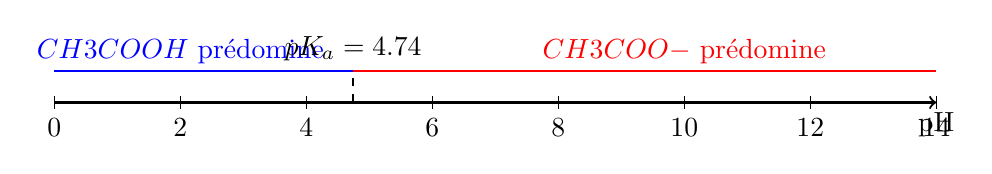
\begin{tikzpicture}[scale=0.8]
\draw[thick,->] (0,0) -- (14,0) node[below] {pH};
\foreach \x in {0,2,4,6,8,10,12,14} {
    \draw (\x,0.1) -- (\x,-0.1) node[below] {\x};
}
\draw[thick,blue] (0,0.5) -- (4.74,0.5);
\draw[thick,red] (4.74,0.5) -- (14,0.5);
\node[blue] at (2,0.8) {$\ce{CH3COOH}$ prédomine};
\node[red] at (10,0.8) {$\ce{CH3COO-}$ prédomine};
\draw[dashed] (4.74,0) -- (4.74,0.5);
\node[above] at (4.74,0.5) {$pK_a = 4.74$};
\end{tikzpicture}
\fig{Diagramme de prédominance du couple acide éthanoïque / ion éthanoate.}
\end{illus}

\begin{exemple}
Pour le couple $\ce{NH4+ / NH3}$ ($pK_a = 9.25$), à pH = 7 (sang humain), quelle espèce prédomine ?
\[
\text{pH} = 7 < 9.25 = pK_a \quad \Rightarrow \quad \text{$\ce{NH4+}$ prédomine.}
\]
\end{exemple}

% ====================================================================
\section{Calcul du pH des solutions aqueuses}
% ====================================================================

\subsection{pH d'un acide fort}

\begin{propriete}[pH d'un acide fort]
Pour une solution d'acide fort de concentration $C_a$ (en $\si{\mol\per\litre}$), la dissociation étant totale :
\[
[\ce{H3O+}] = C_a \quad \Rightarrow \quad \boxed{\text{pH} = -\log C_a}
\]
Cette formule est valable pour $C_a \gtrsim \SI{1e-6}{\mol\per\litre}$.
\end{propriete}

\begin{exemple}
Calculer le pH d'une solution d'acide chlorhydrique $\ce{HCl}$ à $\SI{0.010}{\mol\per\litre}$.
\[
\text{pH} = -\log(0.010) = -\log(10^{-2}) = 2.0
\]
\end{exemple}

\subsection{pH d'une base forte}

\begin{propriete}[pH d'une base forte]
Pour une solution de base forte de concentration $C_b$ (en $\si{\mol\per\litre}$), la dissociation étant totale :
\[
[\ce{HO-}] = C_b \quad \Rightarrow \quad [\ce{H3O+}] = \frac{K_e}{C_b} \quad \Rightarrow \quad \boxed{\text{pH} = 14 + \log C_b}
\]
(à $\SI{25}{\celsius}$). Valable pour $C_b \gtrsim \SI{1e-6}{\mol\per\litre}$.
\end{propriete}

\begin{exemple}
Calculer le pH d'une solution de soude $\ce{NaOH}$ à $\SI{0.0010}{\mol\per\litre}$.
\[
\text{pH} = 14 + \log(0.0010) = 14 + \log(10^{-3}) = 14 - 3 = 11.0
\]
\end{exemple}

\subsection{pH d'un acide faible}

\begin{propriete}[pH d'un acide faible — Approximation]
Pour un acide faible $\ce{HA}$ de concentration $C_a$ et de constante $K_a$, si $C_a \gg [\ce{H3O+}]$ (acide peu dissocié), on peut utiliser l'approximation :
\[
[\ce{H3O+}] \approx \sqrt{K_a \times C_a} \quad \Rightarrow \quad \boxed{\text{pH} \approx \frac{1}{2} \left(pK_a - \log C_a\right)}
\]
Cette approximation est valable si $C_a \gg K_a$ (ou $C_a \gtrsim 100 \times K_a$).
\end{propriete}

\begin{exemple}
Calculer le pH d'une solution d'acide éthanoïque $\ce{CH3COOH}$ à $\SI{0.10}{\mol\per\litre}$ ($pK_a = 4.74$).
\[
\text{pH} \approx \frac{1}{2} \left(4.74 - \log(0.10)\right) = \frac{1}{2} \left(4.74 - (-1)\right) = \frac{1}{2} \times 5.74 = 2.87
\]
\end{exemple}

\begin{remarque}
Pour un acide faible, le pH est toujours supérieur à celui d'un acide fort de même concentration (car la dissociation est partielle).
\end{remarque}

\subsection{pH d'une base faible}

\begin{propriete}[pH d'une base faible — Approximation]
Pour une base faible $\ce{B}$ de concentration $C_b$ et de $pK_a$ du couple $\ce{BH+/B}$, on peut utiliser :
\[
[\ce{HO-}] \approx \sqrt{\frac{K_e}{K_a} \times C_b} \quad \Rightarrow \quad \boxed{\text{pH} \approx 7 + \frac{1}{2} \left(pK_a + \log C_b\right)}
\]
\end{propriete}

\begin{exemple}
Calculer le pH d'une solution d'ammoniac $\ce{NH3}$ à $\SI{0.10}{\mol\per\litre}$ ($pK_a(\ce{NH4+/NH3}) = 9.25$).
\[
\text{pH} \approx 7 + \frac{1}{2} \left(9.25 + \log(0.10)\right) = 7 + \frac{1}{2} \left(9.25 - 1\right) = 7 + \frac{1}{2} \times 8.25 = 7 + 4.125 = 11.125 \approx 11.1
\]
\end{exemple}

\begin{aretenir}
\begin{itemize}
    \item Acide fort : $\text{pH} = -\log C_a$.
    \item Base forte : $\text{pH} = 14 + \log C_b$.
    \item Acide faible : $\text{pH} \approx \frac{1}{2}(pK_a - \log C_a)$.
    \item Base faible : $\text{pH} \approx 7 + \frac{1}{2}(pK_a + \log C_b)$.
\end{itemize}
\end{aretenir}

% ====================================================================
\section{L'essentiel à retenir}
% ====================================================================

\begin{synthese}
\subsection*{Définitions clés}
\begin{itemize}
    \item \textbf{Acide} : espèce qui cède un proton $\ce{H+}$.
    \item \textbf{Base} : espèce qui capte un proton $\ce{H+}$.
    \item \textbf{Couple acide/base} : $\ce{HA / A-}$.
    \item \textbf{Réaction acido-basique} : transfert de proton.
\end{itemize}

\subsection*{Produit ionique de l'eau}
\[
K_e = [\ce{H3O+}] \times [\ce{HO-}] = \num{1.0e-14} \quad (\text{à } \SI{25}{\celsius})
\]

\subsection*{pH}
\[
\text{pH} = -\log[\ce{H3O+}] \quad ; \quad [\ce{H3O+}] = 10^{-\text{pH}}
\]

\subsection*{Constante d'acidité}
\[
K_a = \frac{[\ce{A-}] \times [\ce{H3O+}]}{[\ce{HA}]} \quad ; \quad pK_a = -\log K_a
\]

\subsection*{Diagramme de prédominance}
\begin{itemize}
    \item $\text{pH} < pK_a$ : $\ce{HA}$ prédomine.
    \item $\text{pH} = pK_a$ : $[\ce{HA}] = [\ce{A-}]$.
    \item $\text{pH} > pK_a$ : $\ce{A-}$ prédomine.
\end{itemize}

\subsection*{Formules de pH (solutions diluées, $\SI{25}{\celsius}$)}
\begin{itemize}
    \item Acide fort : $\text{pH} = -\log C_a$.
    \item Base forte : $\text{pH} = 14 + \log C_b$.
    \item Acide faible : $\text{pH} \approx \frac{1}{2}(pK_a - \log C_a)$.
    \item Base faible : $\text{pH} \approx 7 + \frac{1}{2}(pK_a + \log C_b)$.
\end{itemize}

\subsection*{Pièges à éviter}
\begin{itemize}
    \item Ne pas confondre acide fort et concentré.
    \item L'approximation pour acide faible n'est valable que si $C_a \gg K_a$.
    \item Le pH n'est défini que pour $[\ce{H3O+}] \lesssim \SI{0.1}{\mol\per\litre}$.
    \item Toujours vérifier la cohérence : un acide donne pH $< 7$, une base donne pH $> 7$.
\end{itemize}
\end{synthese}

% ====================================================================
\section{Méthodes \& savoir-faire}
% ====================================================================

\methode{Identifier un acide et une base selon Brønsted}
Pour déterminer si une espèce est un acide ou une base, regardez si elle peut perdre ou gagner un proton $\ce{H+}$.
\begin{itemize}
    \item Une espèce qui contient un hydrogène labile (souvent lié à O, N, S) peut être un acide.
    \item Une espèce qui possède un doublet non liant peut être une base.
\end{itemize}
\begin{exemple}
Identifier le rôle de $\ce{HCO3-}$ dans les réactions suivantes :
\begin{itemize}
    \item $\ce{HCO3- + H3O+ -> H2CO3 + H2O}$ : $\ce{HCO3-}$ capte un proton $\Rightarrow$ base.
    \item $\ce{HCO3- + HO- -> CO3^2- + H2O}$ : $\ce{HCO3-}$ cède un proton $\Rightarrow$ acide.
\end{itemize}
\end{exemple}

\methode{Écrire l'équation d'une réaction acido-basique}
\begin{enumerate}
    \item Identifier l'acide (donneur de proton) et la base (accepteur de proton).
    \item Écrire les deux demi-équations : $\ce{Acide1 -> Base1 + H+}$ et $\ce{Base2 + H+ -> Acide2}$.
    \item Additionner les deux demi-équations en simplifiant les $\ce{H+}$.
\end{enumerate}
\begin{exemple}
Réaction entre l'acide éthanoïque $\ce{CH3COOH}$ et l'ammoniac $\ce{NH3}$.
\begin{itemize}
    \item $\ce{CH3COOH -> CH3COO- + H+}$ (acide 1)
    \item $\ce{NH3 + H+ -> NH4+}$ (base 2)
    \item Bilan : $\ce{CH3COOH + NH3 -> CH3COO- + NH4+}$
\end{itemize}
\end{exemple}

\methode{Calculer le pH d'un acide fort}
\begin{enumerate}
    \item Vérifier que l'acide est fort (liste des acides forts).
    \item Utiliser la relation $[\ce{H3O+}] = C_a$.
    \item Appliquer $\text{pH} = -\log C_a$.
\end{enumerate}
\begin{exemple}
Calculer le pH d'une solution d'acide nitrique $\ce{HNO3}$ à $\SI{5.0e-3}{\mol\per\litre}$.
\[
\text{pH} = -\log(5.0 \times 10^{-3}) = -\log 5.0 - \log 10^{-3} = -0.70 + 3 = 2.30
\]
\end{exemple}

\methode{Calculer le pH d'une base forte}
\begin{enumerate}
    \item Vérifier que la base est forte.
    \item Utiliser $[\ce{HO-}] = C_b$.
    \item Calculer $[\ce{H3O+}] = K_e / C_b$.
    \item Appliquer $\text{pH} = -\log[\ce{H3O+}]$ ou $\text{pH} = 14 + \log C_b$.
\end{enumerate}
\begin{exemple}
Calculer le pH d'une solution de potasse $\ce{KOH}$ à $\SI{2.0e-4}{\mol\per\litre}$.
\[
\text{pH} = 14 + \log(2.0 \times 10^{-4}) = 14 + \log 2.0 + \log 10^{-4} = 14 + 0.30 - 4 = 10.30
\]
\end{exemple}

\methode{Calculer le pH d'un acide faible}
\begin{enumerate}
    \item Vérifier que l'acide est faible ($pK_a > 0$).
    \item Vérifier l'approximation : $C_a \gtrsim 100 \times K_a$ (ou $C_a \gg K_a$).
    \item Appliquer $\text{pH} \approx \frac{1}{2}(pK_a - \log C_a)$.
\end{enumerate}
\begin{exemple}
Calculer le pH d'une solution d'acide méthanoïque $\ce{HCOOH}$ à $\SI{0.050}{\mol\per\litre}$ ($pK_a = 3.75$).
\[
\text{pH} \approx \frac{1}{2}(3.75 - \log(0.050)) = \frac{1}{2}(3.75 - (-1.30)) = \frac{1}{2} \times 5.05 = 2.53
\]
Vérification : $C_a = 0.050$, $K_a = 10^{-3.75} = \num{1.78e-4}$, $C_a / K_a \approx 281 > 100$, approximation valable.
\end{exemple}

\methode{Calculer le pH d'une base faible}
\begin{enumerate}
    \item Identifier le $pK_a$ du couple acide/base conjugué ($\ce{BH+/B}$).
    \item Vérifier l'approximation : $C_b \gtrsim 100 \times K_a$ (où $K_a$ est celle du couple $\ce{BH+/B}$).
    \item Appliquer $\text{pH} \approx 7 + \frac{1}{2}(pK_a + \log C_b)$.
\end{enumerate}
\begin{exemple}
Calculer le pH d'une solution d'éthanoate de sodium $\ce{CH3COONa}$ à $\SI{0.20}{\mol\per\litre}$ ($pK_a(\ce{CH3COOH/CH3COO-}) = 4.74$).
\[
\text{pH} \approx 7 + \frac{1}{2}(4.74 + \log(0.20)) = 7 + \frac{1}{2}(4.74 - 0.70) = 7 + \frac{1}{2} \times 4.04 = 7 + 2.02 = 9.02
\]
\end{exemple}

\methode{Utiliser le diagramme de prédominance}
Pour déterminer l'espèce majoritaire à un pH donné :
\begin{enumerate}
    \item Connaître le $pK_a$ du couple.
    \item Comparer le pH au $pK_a$.
    \item Conclure : si pH $< pK_a$, l'acide prédomine ; si pH $> pK_a$, la base prédomine.
\end{enumerate}
\begin{exemple}
Dans le sang humain (pH $\approx 7.4$), quelle est la forme prédominante du couple $\ce{H2CO3/HCO3-}$ ($pK_a = 6.35$) ?
\[
\text{pH} = 7.4 > 6.35 = pK_a \quad \Rightarrow \quad \ce{HCO3-} \text{ prédomine.}
\]
\end{exemple}

\methode{Déterminer le $pK_a$ à partir d'une mesure de pH}
Pour un acide faible $\ce{HA}$ de concentration $C_a$ connue, on mesure le pH de la solution.
\begin{enumerate}
    \item Calculer $[\ce{H3O+}] = 10^{-\text{pH}}$.
    \item En solution, $[\ce{A-}] = [\ce{H3O+}]$ (si on néglige l'autoprotolyse de l'eau).
    \item $[\ce{HA}] \approx C_a - [\ce{H3O+}]$.
    \item Calculer $K_a = \frac{[\ce{A-}] \times [\ce{H3O+}]}{[\ce{HA}]}$ puis $pK_a = -\log K_a$.
\end{enumerate}
\begin{exemple}
Une solution d'acide benzoïque $\ce{C6H5COOH}$ à $\SI{0.10}{\mol\per\litre}$ a un pH de 2.60. Calculer son $pK_a$.
\[
[\ce{H3O+}] = 10^{-2.60} = \SI{2.51e-3}{\mol\per\litre}
\]
\[
[\ce{C6H5COO-}] = [\ce{H3O+}] = \SI{2.51e-3}{\mol\per\litre}
\]
\[
[\ce{C6H5COOH}] = 0.10 - 0.00251 \approx \SI{0.0975}{\mol\per\litre}
\]
\[
K_a = \frac{(2.51 \times 10^{-3})^2}{0.0975} = \frac{6.30 \times 10^{-6}}{0.0975} = \num{6.46e-5}
\]
\[
pK_a = -\log(6.46 \times 10^{-5}) = 4.19
\]
\end{exemple}